% Default 10pt beamer
\documentclass{dt}

\title{Mastering maplib}
\author{Veronika Heimsbakk}

\usepackage{hyperref}
\usepackage{lineno}
\usepackage{color, colortbl}
\usetikzlibrary{shapes}

\usepackage{tgpagella}
\usepackage[small,euler-digits]{eulervm}
\usepackage{amsmath}
\usepackage{tabularx}
\usepackage{makecell}


\tikzstyle{fargeA}=[fill=red,fill opacity=0.3]
\tikzstyle{fargeB}=[fill=blue,fill opacity=0.3]
\tikzstyle{fargeC}=[fill=green,fill opacity=0.3]

\def\mengdeA{(150:1) circle (1.4cm)}
\def\mengdeB{(30:1) circle (1.4cm)}
\def\mengdeC{(-90:1) circle (1.4cm)}

\newcommand{\dxA}{\draw\mengdeA;}
\newcommand{\dxB}{\draw\mengdeB;}
\newcommand{\dxC}{\draw\mengdeC;}

\newcommand{\fxA}{\fill\mengdeA [fargeA];}
\newcommand{\fxB}{\fill\mengdeB [fargeB];}
\newcommand{\fxC}{\fill\mengdeC [fargeC];}

\newcommand{\clA}{\clip\mengdeA;}
\newcommand{\clB}{\clip\mengdeB;}
\newcommand{\clAB}{\clip\mengdeA\mengdeB;}
\newcommand{\clABC}{\clip\mengdeA\mengdeB\mengdeC;}

\newcommand{\nota}[1]{\node[at={(0,3cm)}]{\ensuremath{#1}}}

\tikzstyle{mikro}=[baseline,scale=0.25,line width=0.5pt]


\renewcommand*{\thefootnote}{\faExclamationCircle{}}


\begin{document}

{
\setbeamertemplate{footline}{} 
\begin{frame}
\tp{}
\end{frame}
}
\addtocounter{framenumber}{-1}


\begin{frame}
\vspace{20pt}

\presentationframev{img/veronika.jpeg}{
Knowledge Graph Specialist $|$ Data Treehouse


\vspace{2pt}


\includegraphics[width=3cm]{img/dt.png}


\vspace{10pt}

veronika@data-treehouse.com\\
\\
\faGithub{} veleda\\
\faLinkedin{} vheimsbakk\\
\faGlobeEurope{} veronahe.no

\vspace{10pt}

}

\end{frame}


\begin{frame}{Agenda}

\Large{
DATA TREEHOUSE\\
MAPLIB\\
DATA\\
ONTOLOGIES\\
MAPPING\\
DATALOG\\
SPARQL\\
SHACL\\
}

\vspace{10pt}

{
\normalsize
\faGithub{}  \texttt{\href{https://github.com/DataTreehouse/maplib-masterclass}{DataTreehouse/maplib-masterclass}}
}

\end{frame}


\begin{frame}
\includegraphics[width=6cm]{img/dt.png}
\end{frame}

\begin{frame}{\includegraphics[height=1cm]{img/dt.png}}
Data Treehouse is a Norwegian knowledge graph solutions software company. Our technology is based upon Magnus Bakken's PhD work.

\vspace{5pt}

\scalebox{0.4}{
	\begin{tikzpicture} 
		\begin{scope}
			\clip [rounded corners=1.5cm] (3,0) rectangle coordinate (centerpoint) (6,3); 
			\node [inner sep=0pt] at (centerpoint) {\includegraphics[width=3cm]{img/magnus.jpeg}}; 
		\end{scope}

\node (1) at (9,2) {\Huge{Magnus Bakken}};
\node (1) at (9.25,1) {\Huge{\faLinkedin{} magnusbakken}};


		\begin{scope}
			\clip [rounded corners=1.5cm] (14,0) rectangle coordinate (centerpoint) (17,3); 
			\node [inner sep=0pt] at (centerpoint) {\includegraphics[width=3cm]{img/oivind.jpeg}}; 
		\end{scope}


\node (1) at (19,2) {\Huge{Øivind Rui}};
\node (1) at (20.8,1) {\Huge{\faLinkedin{} øivind-rui-a720492}};


		\begin{scope}
			\clip [rounded corners=1.5cm] (27,0) rectangle coordinate (centerpoint) (30,3); 
			\node [inner sep=0pt] at (centerpoint) {\includegraphics[width=3cm]{img/veronika.jpeg}}; 
		\end{scope}

\node (1) at (33.5,2) {\Huge{Veronika Heimsbakk}};
\node (1) at (32.7,1) {\Huge{\faLinkedin{} vheimsbakk}};


	\end{tikzpicture}
}

\vspace{5pt}

We develop and maintain a series of open source\footnote{\vspace{10pt}Some functionalities are under licensing.} frameworks for Python.

\begin{itemize}
\item \tikz{\node[fill=dtgreen] (1) at (0,-0.2) {\textbf{maplib}};} build and enrich harmonized knowledge graphs from any sources.
\item \textbf{chrontext}: semantic integration technology that protect your existing platforms and infrastructure while leveraging the value of data.
\item \textbf{querymesh}: context-enabled queries over analytical data sets provides the first level of querymesh, the Operational Data Mesh, where data products are created, maintained and managed.
\end{itemize}

\end{frame}


\begin{frame}
\begin{center}
\includegraphics[width=0.6\textwidth]{img/stack-2.png}
\end{center}
\end{frame}

\begin{frame}{maplib at a glance}

maplib is developed in Rust on \textit{Polars} and \textit{Apache Arrow}, and available as Python frameworks.

\vspace{10pt}

\begin{minipage}{0.45\textwidth}
\begin{tikzpicture}

\draw[rounded corners, fill=dtgreen!30] (0,3.75) rectangle (5,4.75);
\node[align=left] (1) at (1.5,4.25) {Knowledge Graph};
\node[align=left] (1) at (4,4.25) {\includegraphics[height=0.5cm]{img/rdf.png} \includegraphics[height=0.5cm]{img/shacl.png} \includegraphics[height=0.5cm]{img/sparql.png}};

\draw[rounded corners, fill=dtgreen!20] (0,2.5) rectangle (5,3.5);
\node[align=left] (1) at (0.9,3) {Mapping};
\node[align=left] (1) at (4,3) {\includegraphics[height=0.6cm]{img/ottr.jpg}};

\draw[rounded corners, fill=dtgreen!10] (0,1.25) rectangle (5,2.25);
\node[align=left] (1) at (1.9,1.75) {Data Engineering tools};
\node[align=left] (1) at (4,1.75) {\includegraphics[height=0.45cm]{img/Pandas.png} \includegraphics[height=0.5cm]{img/polar.png}};

\draw[rounded corners, draw=dtgreen] (0,0) rectangle (5,1);
\node[] (1) at (2.25,0.5) {Data Sources \hspace{5pt} \textcolor{dtgreen}{\faCloud{} \faFileCsv{} \faFileCode{} $\cdots$ \faDatabase{}}};

\end{tikzpicture}
\end{minipage}
\begin{minipage}{0.45\textwidth}
\textbf{Knowledge Graph} Support for most knowledge graph operations, as RDF Model, SPARQL, SHACL, and Datalog reasoning.\\
\\
\textbf{Mapping} Template based mapping using Reasonable Ontology Templates (OTTR). Serialise data frames to RDF in no time!\\
\\
\textbf{Data Engineering tools} maplib supports instance data handling with \textit{data frames} in Python by core.\\
\\
\textbf{Data Sources} data bist data. 

\end{minipage}

\vspace{10pt}

\textbf{Check out:} \url{https://datatreehouse.github.io/maplib}

\end{frame}

%%%%%%%%%%%%%%%%%%%%%%%%%%%%%%%%%%% DATA

\begin{frame}
\Huge{\textbf{DATA}}
\end{frame}

\begin{frame}

\begin{center}
\includegraphics[width=0.75\textwidth]{img/moons.png}
\includegraphics[width=0.75\textwidth]{img/planets.png}
\end{center}

\begin{itemize}
\item[\faGithub{}] \texttt{\href{https://github.com/devstronomy/nasa-data-scraper/tree/master}{devstronomy/nasa-data-scraper}}
\end{itemize}

\end{frame}

\begin{frame}
\includegraphics[width=0.8\textwidth]{img/sticker.png}
\end{frame}



\begin{frame}[fragile]{Data frames}
\includegraphics[width=0.3\textwidth]{img/polars.png}\\
\faGlobeEurope{} \texttt{\url{https://pola.rs/}}

\begin{code}
\begin{verbatim}
  df_planets = pl.read_csv("data/planets.csv")

  # Create URI for subject
  df_planets = df_planets.with_columns(
    (ns + pl.col("planet")).alias("planet_uri")
  )
\end{verbatim}
\end{code}

\end{frame}

\begin{frame}[fragile]{Data frames}

\begin{code}
\begin{verbatim}
  df_planets = df_planets.select(
    ["planet", 
    "planet_uri", # the new column we just made :-)
    "mean_temperature",
    "length_of_day",
    "orbital_period"]
  )
\end{verbatim}
\end{code}
\end{frame}


\begin{frame}{Planets}

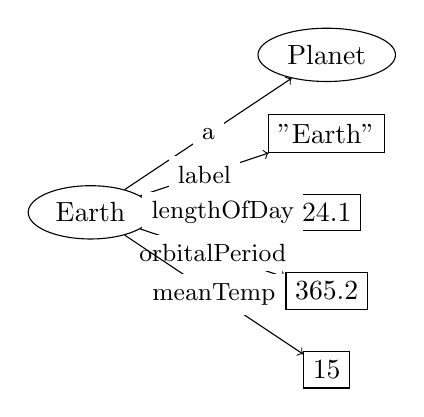
\begin{tikzpicture}
\node[ellipse, draw=black] (1) at (0,-2) {Earth};
\node[ellipse, draw=black] (2) at (3,0) {Planet};
\node[rectangle, draw=black] (3) at (3,-1) {"Earth"};
\node[rectangle, draw=black] (4) at (3,-2) {24.1};
\node[rectangle, draw=black] (5) at (3,-3) {365.2};
\node[rectangle, draw=black] (55) at (3,-4) {15};

\draw[->] (1) --node[fill=white, font=\small] {a} (2);
\draw[->] (1) --node[fill=white, font=\small] {label} (3);
\draw[->] (1) --node[fill=white, font=\small] {lengthOfDay} (4);
\draw[->] (1) --node[fill=white, font=\small] {orbitalPeriod} (5);
\draw[->] (1) --node[fill=white, font=\small] {meanTemp} (55);
\end{tikzpicture}

\end{frame}

\begin{frame}[fragile]{Data frames---satellites}

\begin{code}
\begin{verbatim}
  df_satellites = pl.read_csv("data/satellites.csv")

  df_satellites = df_satellites.with_columns(
    (ns + pl.col("planet")).alias("planet_uri")
  )

  df_satellites = df_satellites.with_columns(
    (ns + pl.col("name")
    .str.replace_all("/", "-"))
    .str.replace_all(" ", "-")
    .alias("satellite_uri")
  )
\end{verbatim}
\end{code}

\end{frame}

\begin{frame}{...with their satellites}

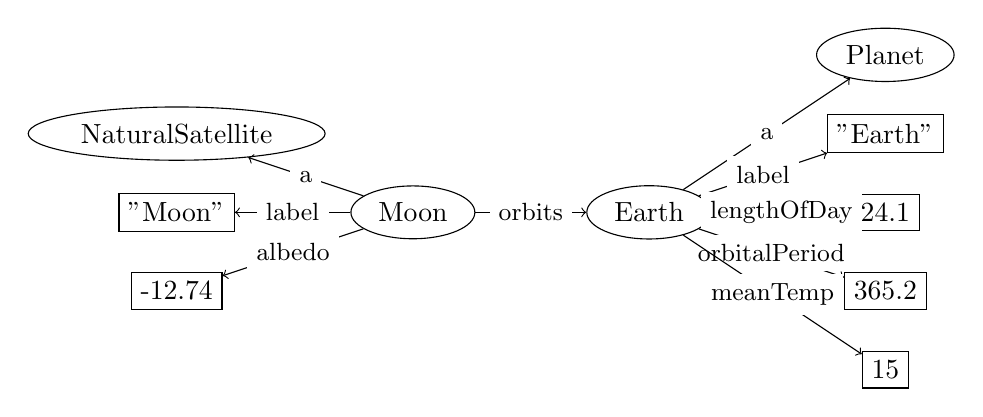
\begin{tikzpicture}
\node[ellipse, draw=black] (1) at (0,-2) {Earth};
\node[ellipse, draw=black] (2) at (3,0) {Planet};
\node[rectangle, draw=black] (3) at (3,-1) {"Earth"};
\node[rectangle, draw=black] (4) at (3,-2) {24.1};
\node[rectangle, draw=black] (5) at (3,-3) {365.2};
\node[rectangle, draw=black] (55) at (3,-4) {15};
\node[ellipse, draw=black] (6) at (-3,-2) {Moon};
\node[rectangle, draw=black] (7) at (-6,-2) {"Moon"};
\node[rectangle, draw=black] (8) at (-6,-3) {-12.74};
\node[ellipse, draw=black] (9) at (-6,-1) {NaturalSatellite};

\draw[->] (1) --node[fill=white, font=\small] {a} (2);
\draw[->] (1) --node[fill=white, font=\small] {label} (3);
\draw[->] (1) --node[fill=white, font=\small] {lengthOfDay} (4);
\draw[->] (1) --node[fill=white, font=\small] {orbitalPeriod} (5);
\draw[->] (1) --node[fill=white, font=\small] {meanTemp} (55);

\draw[->] (6) --node[fill=white, font=\small] {orbits} (1);
\draw[->] (6) --node[fill=white, font=\small] {label} (7);
\draw[->] (6) --node[fill=white, font=\small] {albedo} (8);
\draw[->] (6) --node[fill=white, font=\small] {a} (9);
\end{tikzpicture}

\end{frame}

%%%%%%%%%%%%%%%%%%%%%%%%%%%%%%%%%%%


%%%%%%%%%%%%%%%%%%%%%%%%%%%%%% MAPPING

\begin{frame}
\Huge{\textbf{MAPPING}}
\end{frame}

\begin{frame}{Reasonable Ontology Templates}

\textbf{maplib} currently support mapping using OTTR\footnote{\vspace{10pt} \textit{ On the roadmap:} RML and SPARQL Anything. \faGrinHearts[regular] }

\vspace{5pt}

\begin{minipage}{0.10\textwidth}
\includegraphics[width=\textwidth]{img/ottr.jpg}
\end{minipage}
\hspace{5pt}
\begin{minipage}{0.65\textwidth}
\textbf{Reasonable Ontology Templates (OTTR)}\\
Aims to provide lightweight syntax for defining templates for RDF.\\Serialising chunks of data in a defined pattern. \faGlobeEurope{} \texttt{\url{https://ottr.xyz/}}
\end{minipage}

\vspace{15pt}

We're diving into stOTTR (Terse Syntax for Reasonable Ontology Template):
\begin{itemize}
\item terms
\item types
\item instances
\item template example
\end{itemize}
\end{frame}

\begin{frame}[fragile]{stOTTR terms}
A term is, syntactically, either a variable, a constant or a list of terms.

\begin{code}
\begin{verbatim}
  ?planet_uri
  ?PLANET

  <http://data-treehouse.com/example>
  ex:mean_temperature

  []
  _:b

  "Jupiter"
  "4879"^^xsd:integer
  57.9
  5427
  true

  ("Phobos", "Deimos")
  (("Phobos", "Deimos"), ex:Mars, (0.642))
\end{verbatim}
\end{code}
\end{frame}

\begin{frame}[fragile]{stOTTR types}
A type, like the type of a term, is either a basic type, or a list type.

\begin{code}
\begin{verbatim}
  xsd:double
  owl:Class
  rdfs:Resource
  ottr:IRI

  List<xsd:string>
  List<NEList<xsd:integer>>
\end{verbatim}
\end{code}
\end{frame}

\begin{frame}[fragile]{stOTTR instances}

stOTTR instances are instructions on how instance data will be serialised. We populate template signatures with actual data.

\begin{code}
\begin{verbatim}
  ottr:Triple(:subject, :predicate, :object) .
  tpl:Satellite(ex:Mars, ex:Phobos) .
  tpl:Star( , ) .
  cross | tpl:Planet(ex:Mercury, ++("Merkur"@no, "Mercury"@en)) .
\end{verbatim}
\end{code}
\end{frame}


\begin{frame}[fragile]{stOTTR template example}

Remember our \texttt{df\_planet} data frame, with selected columns: \texttt{planet}, \texttt{planet\_uri}, \texttt{mean\_temperature}, \texttt{length\_of\_day}, and \texttt{orbital\_period}. \textbf{Template parameters must have the same name as data frame column headers.}

\begin{code}
\begin{verbatim}
  tpl:Planet[
    ! ottr:IRI ?planet_uri , 
    xsd:string ?planet ,
    ?mean_temperature ,
    ? ?length_of_day ,
    ?orbital_period
  ] :: {
    ottr:Triple(?planet_uri, rdf:type, :Planet), 
    ottr:Triple(?planet_uri, rdf:type, owl:NamedIndividual),
    ottr:Triple(?planet_uri, rdfs:label, ?planet),
    ottr:Triple(?planet_uri, :meanTemperature, ?mean_temperature),
    ottr:Triple(?planet_uri, :lengthOfDay, ?length_of_day),
    ottr:Triple(?planet_uri, :orbitalPeriod, ?orbital_period)
  } .
\end{verbatim}
\end{code}
\end{frame}

\begin{frame}[fragile]{Need to kick-start your template?}

With \textbf{maplib}, you can generate a stOTTR template based on your data frame. A perfect starting point for kicking off your template, so that you can focus on fine-tuning instead of layout.

\begin{code}
\begin{verbatim}
  tmp_tpl = m.expand_default(df_planets, "planet_uri")
\end{verbatim}
\end{code}

\texttt{m.expand\_default} takes the data frame, and the column containing subject URI as parameters, and returns a string containing the stOTTR template.

\end{frame}


\begin{frame}[fragile]{Mapping your data frame using OTTR}

At core in \textbf{maplib}, is the mapping (surprise!). 

\begin{code}
\begin{verbatim}
  with open("tpl.ttl", "r") as file:
    tpl = file.read()

  # Init a model, and add template
  m = Model()
  m.add_template(tpl)

  # Mapping: serialise data frame to RDF using templates
  m.map("http://data.treehouse.example/tpl/Planet", df_planets())
\end{verbatim}
\end{code}

\begin{itemize}
\item \texttt{m.add\_template()} takes in the template as string or programmatically constructed \texttt{Template}.
\item \texttt{m.map()} takes in template URI and the data frame to be serialised.
\end{itemize}

\end{frame}


\begin{frame}[fragile]{Results of mapping}


\textbf{Serialisation}

Using \texttt{m.write(output\_file, format)} one can serialise \texttt{m} and write to file.\\Supported formats: \texttt{"ntriples"}, \texttt{"turtle"}, and \texttt{"rdf/xml"}\footnote{\vspace{10pt}\textit{ On the roadmap:} JSON-LD, pretty ttl}
\vspace{5pt}

\begin{code}
\begin{verbatim}
  dt:Jupiter a dt:Planet,
    owl:NamedIndividual ;
  rdfs:label "Jupiter" ;
  dt:lengthOfDay 9.9e+00 ;
  dt:meanTemperature "-110"^^xsd:long ;
  dt:orbitalPeriod 4.331e+03 .
\end{verbatim}
\end{code}

\end{frame}


%%%%%%%%%%%%%%%%%%%%%%%%%%%%%%%%%%%


%%%%%%%%%%%%%%%%%%%%%%%%%%%% ONTOLOGY

\begin{frame}
\Huge{\textbf{ONTOLOGY}}
\end{frame}

\begin{frame}{}

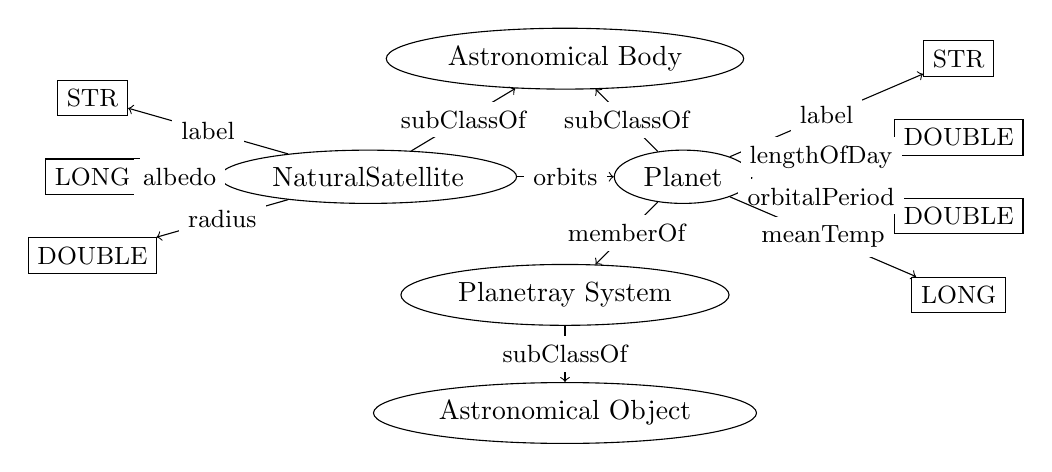
\begin{tikzpicture}
\node[ellipse, draw=black] (1) at (0,-2.5) {Planet};
\node[rectangle, draw=black] (3) at (3.5,-1) {\small{STR}};
\node[rectangle, draw=black] (4) at (3.5,-2) {\small{DOUBLE}};
\node[rectangle, draw=black] (5) at (3.5,-3) {\small{DOUBLE}};
\node[rectangle, draw=black] (55) at (3.5,-4) {\small{LONG}};
\node[ellipse, draw=black] (6) at (-4,-2.5) {NaturalSatellite};
\node[rectangle, draw=black] (7) at (-7.5,-1.5) {\small{STR}};
\node[rectangle, draw=black] (8) at (-7.5,-2.5) {\small{LONG}};
\node[rectangle, draw=black] (9) at (-7.5,-3.5) {\small{DOUBLE}};


\draw[->] (1) --node[fill=white, font=\small] {label} (3);
\draw[->] (1) --node[fill=white, font=\small] {lengthOfDay} (4);
\draw[->] (1) --node[fill=white, font=\small] {orbitalPeriod} (5);
\draw[->] (1) --node[fill=white, font=\small] {meanTemp} (55);

\draw[->] (6) --node[fill=white, font=\small] {orbits} (1);
\draw[->] (6) --node[fill=white, font=\small] {label} (7);
\draw[->] (6) --node[fill=white, font=\small] {albedo} (8);
\draw[->] (6) --node[fill=white, font=\small] {radius} (9);


\node[ellipse, draw=black] (ab) at (-1.5,-1) {Astronomical Body};
\draw[->] (1) --node[fill=white, font=\small] {subClassOf} (ab);
\draw[->] (6) --node[fill=white, font=\small] {subClassOf} (ab);

\node[ellipse, draw=black] (ps) at (-1.5,-4) {Planetray System};
\node[ellipse, draw=black] (ao) at (-1.5,-5.5) {Astronomical Object};
\draw[->] (ps) --node[fill=white, font=\small] {subClassOf} (ao);
\draw[->] (1) --node[fill=white, font=\small] {memberOf} (ps);
\end{tikzpicture}

\end{frame}


\begin{frame}{}

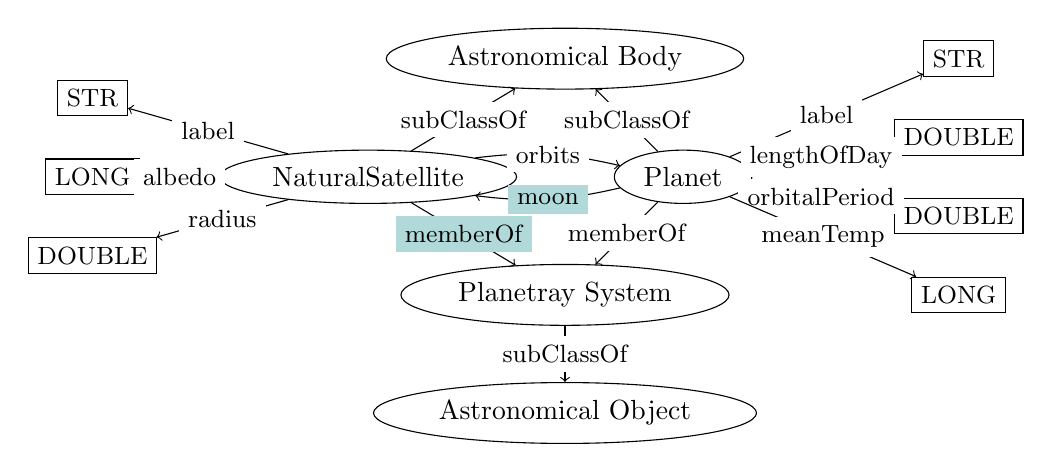
\begin{tikzpicture}
\node[ellipse, draw=black] (1) at (0,-2.5) {Planet};
\node[rectangle, draw=black] (3) at (3.5,-1) {\small{STR}};
\node[rectangle, draw=black] (4) at (3.5,-2) {\small{DOUBLE}};
\node[rectangle, draw=black] (5) at (3.5,-3) {\small{DOUBLE}};
\node[rectangle, draw=black] (55) at (3.5,-4) {\small{LONG}};
\node[ellipse, draw=black] (6) at (-4,-2.5) {NaturalSatellite};
\node[rectangle, draw=black] (7) at (-7.5,-1.5) {\small{STR}};
\node[rectangle, draw=black] (8) at (-7.5,-2.5) {\small{LONG}};
\node[rectangle, draw=black] (9) at (-7.5,-3.5) {\small{DOUBLE}};


\draw[->] (1) --node[fill=white, font=\small] {label} (3);
\draw[->] (1) --node[fill=white, font=\small] {lengthOfDay} (4);
\draw[->] (1) --node[fill=white, font=\small] {orbitalPeriod} (5);
\draw[->] (1) --node[fill=white, font=\small] {meanTemp} (55);

\draw[->, bend left=10] (6) to node[fill=white, font=\small] {orbits} (1);
\draw[->, bend left=10] (1) to node[fill=teal!30, font=\small] {moon} (6);
\draw[->] (6) --node[fill=white, font=\small] {label} (7);
\draw[->] (6) --node[fill=white, font=\small] {albedo} (8);
\draw[->] (6) --node[fill=white, font=\small] {radius} (9);


\node[ellipse, draw=black] (ab) at (-1.5,-1) {Astronomical Body};
\draw[->] (1) --node[fill=white, font=\small] {subClassOf} (ab);
\draw[->] (6) --node[fill=white, font=\small] {subClassOf} (ab);

\node[ellipse, draw=black] (ps) at (-1.5,-4) {Planetray System};
\node[ellipse, draw=black] (ao) at (-1.5,-5.5) {Astronomical Object};
\draw[->] (ps) --node[fill=white, font=\small] {subClassOf} (ao);
\draw[->] (1) --node[fill=white, font=\small] {memberOf} (ps);
\draw[->] (6) --node[fill=teal!30, font=\small] {memberOf} (ps);
\end{tikzpicture}

\end{frame}


%%%%%%%%%%%%%%%%%%%%%%%%%%%%%%%%%%%


%%%%%%%%%%%%%%%%%%%%%%%%%%%%%%%%%%%%

\begin{frame}
\Huge{\textbf{SPARQL}}
\end{frame}

\begin{frame}[fragile]{m.query}

\textbf{Count}

\vspace{5pt}

\texttt{m.query()} returns a data frame containing the query result. The bound variable \texttt{?count} is the column header in this example, and can be fetched using \texttt{["count"][0]} for first cell of first row in column \texttt{count}.

\begin{code}
\begin{verbatim}
  # Print number of triples
  count = """SELECT (COUNT(?s) AS ?count) WHERE { ?s ?p ?o . }"""
  print("Graph size after mapping: ", m.query(count)["count"][0])
\end{verbatim}
\end{code}

\end{frame}


\begin{frame}[fragile]{m.insert}

\begin{code}
\begin{verbatim}
  # Insert everything that has some rdf:type to anything except for owl:Class 
  # to be rdf:type of owl:NamedIndividual

  CONSTRUCT {
    ?s rdf:type owl:NamedIndividual .
  }  
  WHERE {
    ?s rdf:type ?o .
    FILTER(?o != owl:Class)
  }
\end{verbatim}
\end{code}

\begin{tikzpicture}
\node[ellipse, draw=black] (1) at (0,0) {Mars};
\node[ellipse, draw=black] (2) at (3,0) {Planet};
\node[ellipse, draw=black] (3) at (6,0) {owl:Class};
\node[ellipse, draw=black, fill=dtgreen!50] (4) at (4,-1) {owl:NamedIndividual};

\draw[->] (1) --node[fill=white] {a} (2);
\draw[->] (2) --node[fill=white] {a} (3);
\draw[->] (1) --node[fill=dtgreen!50] {a} (4);

\end{tikzpicture}


\end{frame}



\begin{frame}[fragile]{m.insert}

\texttt{m.insert()} expect a SPARQL \texttt{CONSTRUCT} query as string, and inserts the constructed statements to the \texttt{Model}.


\begin{code}
\begin{verbatim}
  with open("queries/insert_individual.rq", "r") as file:
    insert_individual = file.read()

  m.insert(insert_individual)
\end{verbatim}
\end{code}

\end{frame}



%%%%%%%%%%%%%%%%%%%%%%%%%%%%%%%%%%%%%



%%%%%%%%%%%%%%%%%%%%%%%%%%%% DATALOG

\begin{frame}
\Huge{\textbf{DATALOG}}
\end{frame}

\begin{frame}{What is Datalog?}
\textbf{Datalog} is a declarative logic programming language. It's a bit similar to Prolog, but resembles more a query language than Prolog does.

\vspace{10pt}

In \textbf{maplib}, Datalog is used for \textit{logical inference} over the knowledge graph\footnote{\vspace{10pt}\textit{ On the roadmap:} RDFS eintailment}.
\end{frame}

\begin{frame}[fragile]{Declaring statements}
\begin{code}
\begin{verbatim}
  [?x, :moon, ?y] :- [?y, :orbits, ?x] .
\end{verbatim}
\end{code}

\vspace{10pt}

\begin{tikzpicture}
\node[ellipse, draw=black] (1) at (0,0) {Phobos};
\node[ellipse, draw=black] (2) at (3,0) {Mars};
\draw[->] (1) --node[fill=white]{orbits} (2) ;
\draw[->, bend left] (2) to node[fill=dtgreen!50]{moon} (1) ;
\end{tikzpicture}

\end{frame}

\begin{frame}[fragile]{Declaring statements}
\begin{code}
\begin{verbatim}
  [?x, :memberOf, ?z] :- [?x, :orbits, ?y], [?y, :memberOf, ?z] .
\end{verbatim}
\end{code}

\vspace{10pt}


\begin{tikzpicture}
\node[ellipse, draw=black] (1) at (0,0) {Phobos};
\node[ellipse, draw=black] (2) at (3,0) {Mars};
\node[ellipse, draw=black] (3) at (8,0) {SolarSystem};
\draw[->] (1) --node[fill=white]{orbits} (2) ;
\draw[->] (2) --node[fill=white]{memberOf} (3) ;
\draw[->, bend right] (1) to node[fill=dtgreen!50]{memberOf} (3) ;
\end{tikzpicture}

\end{frame}


\begin{frame}[fragile]{Declaring statements}
\begin{code}
\begin{verbatim}
  [?x, :memberOf, ?z] :- [?x, :orbits, ?y], [?y, :memberOf, ?z] .
\end{verbatim}
\end{code}

\vspace{10pt}


\begin{tikzpicture}
\node[ellipse, draw=black] (0) at (-3,0) {XYZ};
\node[ellipse, draw=black] (1) at (0,0) {Phobos};
\node[ellipse, draw=black] (2) at (3,0) {Mars};
\node[ellipse, draw=black] (3) at (8,0) {SolarSystem};
\draw[->] (0) --node[fill=white]{orbits} (1) ;
\draw[->] (1) --node[fill=white]{orbits} (2) ;
\draw[->] (2) --node[fill=white]{memberOf} (3) ;
\draw[->, bend right] (1) to node[fill=white]{memberOf} (3) ;
\draw[->, bend right] (0) to node[fill=dtgreen!50]{memberOf} (3) ;
\end{tikzpicture}

\end{frame}


\begin{frame}[fragile]{Classification}
\begin{code}
\begin{verbatim}
  [?planet, rdf:type, :TemperateWorld] :- 
    [?planet, rdf:type, :Planet] , 
    [?planet, :meanTemperature, ?temp] ,
    FILTER(?temp >= -100 && ?temp <= 100) .
\end{verbatim}
\end{code}

\vspace{10pt}

All things that are \textit{Temperate World}s are things that are of type \texttt{Planet}, and has a \texttt{meanTemperature} between \texttt{-100} and \texttt{100}.

\vspace{10pt}

\begin{tikzpicture}
\node[ellipse, draw=black] (1) at (0,0) {Mars};
\node[ellipse, draw=black] (2) at (3,0) {Planet};
\node[rectangle, draw=black] (3) at (3,-1) {-65};
\node[ellipse, draw=black] (4) at (3,1) {TemperateWorld};
\draw[->] (1) --node[fill=white]{a} (2);
\draw[->] (1) --node[fill=white]{meanTemperature} (3);
\draw[->] (1) --node[fill=dtgreen!50]{a} (4);
\end{tikzpicture}

\end{frame}


\begin{frame}[fragile]{infer in maplib}
\begin{code}
\begin{verbatim}
  with open("ttl/rule.dlog", "r") as file:
    rules = file.read()

  m.infer(rules)
\end{verbatim}
\end{code}
\end{frame}


\begin{frame}[fragile]{Result after reasoning}
\begin{code}
\begin{verbatim}
  dt:Mars a dt:Planet,
    dt:TemperateWorld, owl:NamedIndividual ; #
    rdfs:label "Mars" ;
    dt:lengthOfDay 2.47e+01 ;
    dt:meanTemperature "-65"^^xsd:long ;
    dt:memberOf dt:SolarSystem ;
    dt:moon dt:Deimos, dt:Phobos ; #
    dt:orbitalPeriod 6.87e+02 .

  dt:Deimos a dt:NaturalSatellite, owl:NamedIndividual ;
    rdfs:label "Deimos" ;
    dt:memberOf dt:SolarSystem ; #
    dt:orbits dt:Mars . 
\end{verbatim}
\end{code}
\end{frame}


%%%%%%%%%%%%%%%%%%%%%%%%%%%%%%%%%%%


%%%%%%%%%%%%%%%%%%%%%%%%%%%%%%%%%%%%

\begin{frame}
\Huge{\textbf{SHACL}}
\end{frame}

\begin{frame}


\begin{center}
\includegraphics[width=0.6\textwidth]{img/benchmark.png}
\end{center}
\faGithub{} oeg-upm/ERA-SHACL-Benchmark


\end{frame}


\begin{frame}[fragile]{Constraining \texttt{:memberOf}}

Astronomical bodies shall be a member of either a planetary system or a star cluster.

\begin{code}
\begin{verbatim}
  rule:AstronomicalBody a sh:NodeShape ;
    sh:targetClass :AstronomicalBody ;
    sh:property rule:AstronomicalBody-memberOf .

  rule:AstronomicalBody-memberOf a sh:PropertyShape ;
    sh:path :memberOf ;
    sh:minCount 1 ;
    sh:or (
        [ sh:class :PlanetarySystem ]
        [ sh:class :StarCluster ]
    ) .
\end{verbatim}
\end{code}

\end{frame}



%%%%%%%%%%%%%%%%%%%%%%%%%%%%%%%%%%%%%

%%%%%%%%%%%%%%%%%%%%%%%%%%%%%%%%%%%%%

\begin{frame}
\Huge{\textbf{TREEHOUSE EXPLORER}}
\end{frame}

\begin{frame}{}
\includegraphics[width=\textwidth]{img/ex2.png}
\end{frame}

%%%%%%%%%%%%%%%%%%%%%%%%%%%%%%%%%%%%%

%%%%%%%%%%%%%%%%%%%%%%%%%%%%%%%%%%%%%


\begin{frame}
\Huge{\textbf{EXPLORE MAPLIB! \textcolor{dtyellow}{\faStar}}}
\end{frame}

\begin{frame}[fragile]{Connected Data London sandbox}

\begin{minipage}{0.45\textwidth}
\textbf{Sanbox environment:} demo.data-treehou.se

\vspace{10pt}

\textbf{\faGithub{} DataTreehouse/maplib-masterclass}

\vspace{10pt}

\begin{code}
\begin{verbatim}
pip install maplib
\end{verbatim}
\end{code}
\end{minipage}
\begin{minipage}{0.45\textwidth}
\begin{tikzpicture}
\draw[rounded corners, fill=dtgreen!30, draw=none] (0,0) rectangle (3,4);
\node[align=center] (1) at (1.5,3.4) {\textbf{MAPLIB}\\ \small{FREE \& OPEN-SOURCE}};
\node[align=left] (2) at (1.25, 2) {I/O\\RDF Model\\SPARQL\\OTTR Mapping};


\draw[rounded corners, fill=dtgreen!30, draw=none] (3.5,0) rectangle (6.5,4);
\node[align=center] (1) at (5,3.4) {\textbf{MAPLIB+}\\ \small{€990/month}};
\node[align=left] (2) at (5.1,1.55) {I/O\\RDF Model\\SPARQL\\OTTR Mapping\\Datalog\\SHACL\\Treehouse explorer};
\end{tikzpicture}

\vspace{5pt}

Early bird (in 2025): €445/month for life.\\
30 day free trial. 
Academic license always free.
\end{minipage}

\end{frame}

\end{document}